\documentclass[10pt]{beamer}

% Balíčky
\usepackage[czech]{babel}
\usepackage{bchart}

% Makra
\newcommand{\resources}{Resources/}

% Nastavení beamer titlepage
\title{Vývoj akční videohry zasazené do prostředí FM}
\subtitle{Bakalářský projekt}
\author{Radek Mocek}
\date{\today}

% Beamer template
\input{\resources beamerTemplate}

% Začátek prezentace
\begin{document}
	
	% Titulní strana
	{
	\setbeamertemplate{footline}{} % Titulní strana bez patičky
	\frame[noframenumbering]{\titlepage} % Nepočítat do celkového počtu framů
	}
	
	% Obsah
%	\begin{frame}{Obsah prezentace}
%		\tableofcontents
%	\end{frame}	

	% Slide 0 :: Zadání
	\section{Zadání} % Tohle je zde kvůli případnému obsahu
	\begin{frame}{Zadání} % Slide a jeho napdpis
		\begin{enumerate} \setlength\itemsep{10pt} % Číslovaný seznam
			\item Rešerše 2D tvorby v Unity
			\item Návrh videohry
			\item Umělá inteligence pro nepřátele, FSM
			\item Implementace, FM zasazení
			\item Zhodnocení
		\end{enumerate}
	\end{frame}

	% Slide 1 :: Motivace
	\section{Motivace}
	\begin{frame}{Motivace}
		\begin{itemize}\setlength\itemsep{10pt} % Nečíslovaný seznam
			\item Záliba ve videohrách
			\item Rozmanitost herního vývoje
			\item Unity $\implies$ C\#
		\end{itemize}
	\end{frame}
	
	% Slide 2 :: Unity obecně
	\section{Unity}
	\begin{frame}{Unity}
		\begin{itemize}\setlength\itemsep{10pt}
			\item Herní engine, 2D i 3D tvorba
			\item 2005, Unity Technologies, closed source
		\end{itemize}
		\vfill
		\begin{bchart}[max=108,plain,unit=\ 000,scale=1.2]
			\bcbar[text=Unity,color=gray!40!white]{108}
			\bcbar[text=Construct,color=teal!40!white]{32}
			\bcbar[text=GM:S,color=green!40!white]{15}
			\bcbar[text=Godot,color=blue!40!white]{14}
			\bcxlabel{Počet projektů v daném enginu na itch.io (zaokrouhleno na tisíce)}
		\end{bchart}
	\end{frame}
	
	% Slide 3 :: Unity obrázek
	% >> Zmínit komponenty, C#, IDE
	\begin{frame}[plain]
			\makebox[\linewidth]{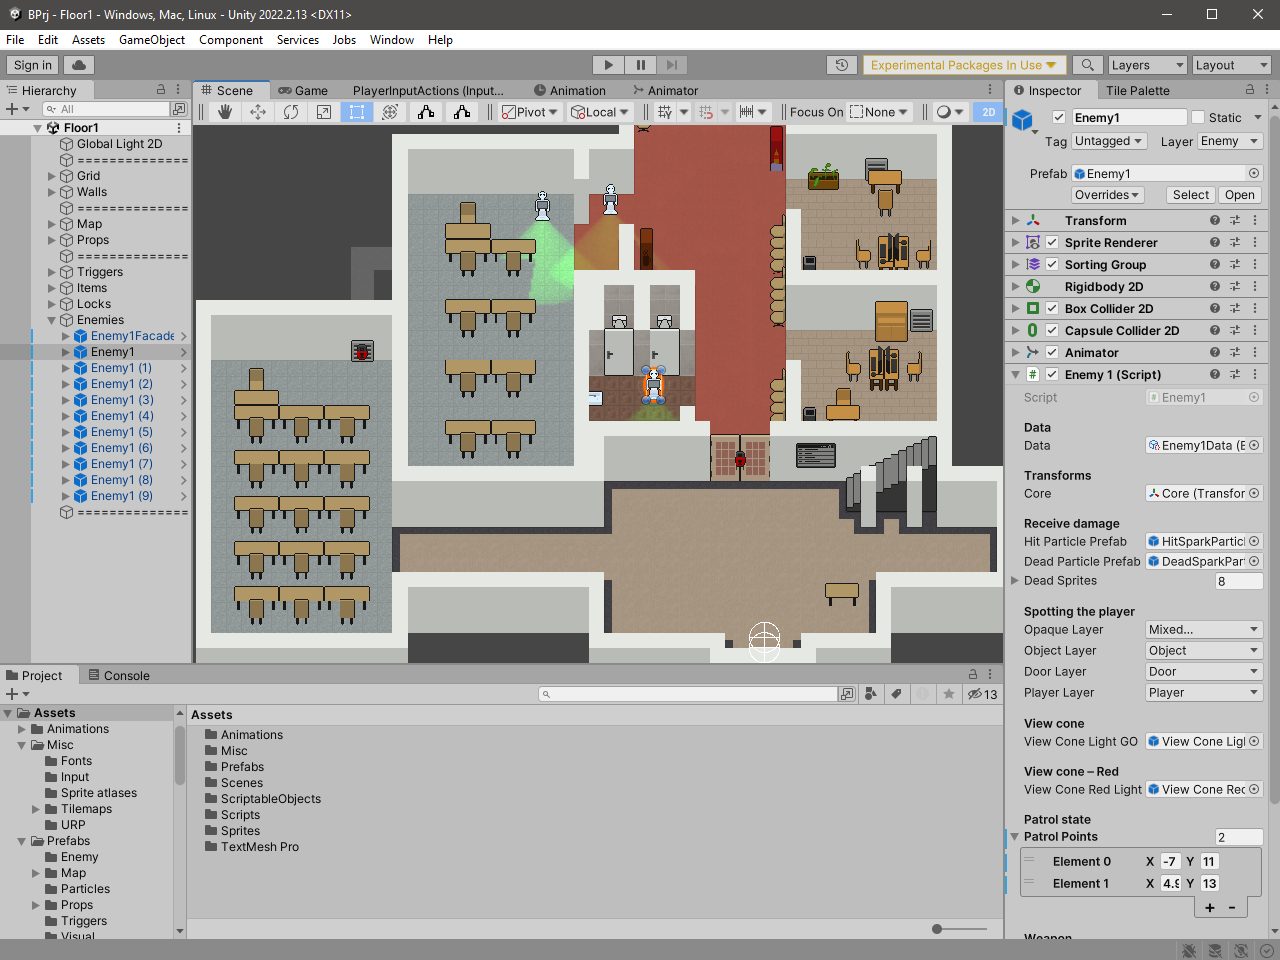
\includegraphics[width=\paperwidth]{Images/Unity}}
	\end{frame}
	
	% Slide 4 :: Unity 2D showcase
	\begin{frame}[plain]
		\makebox[\linewidth]{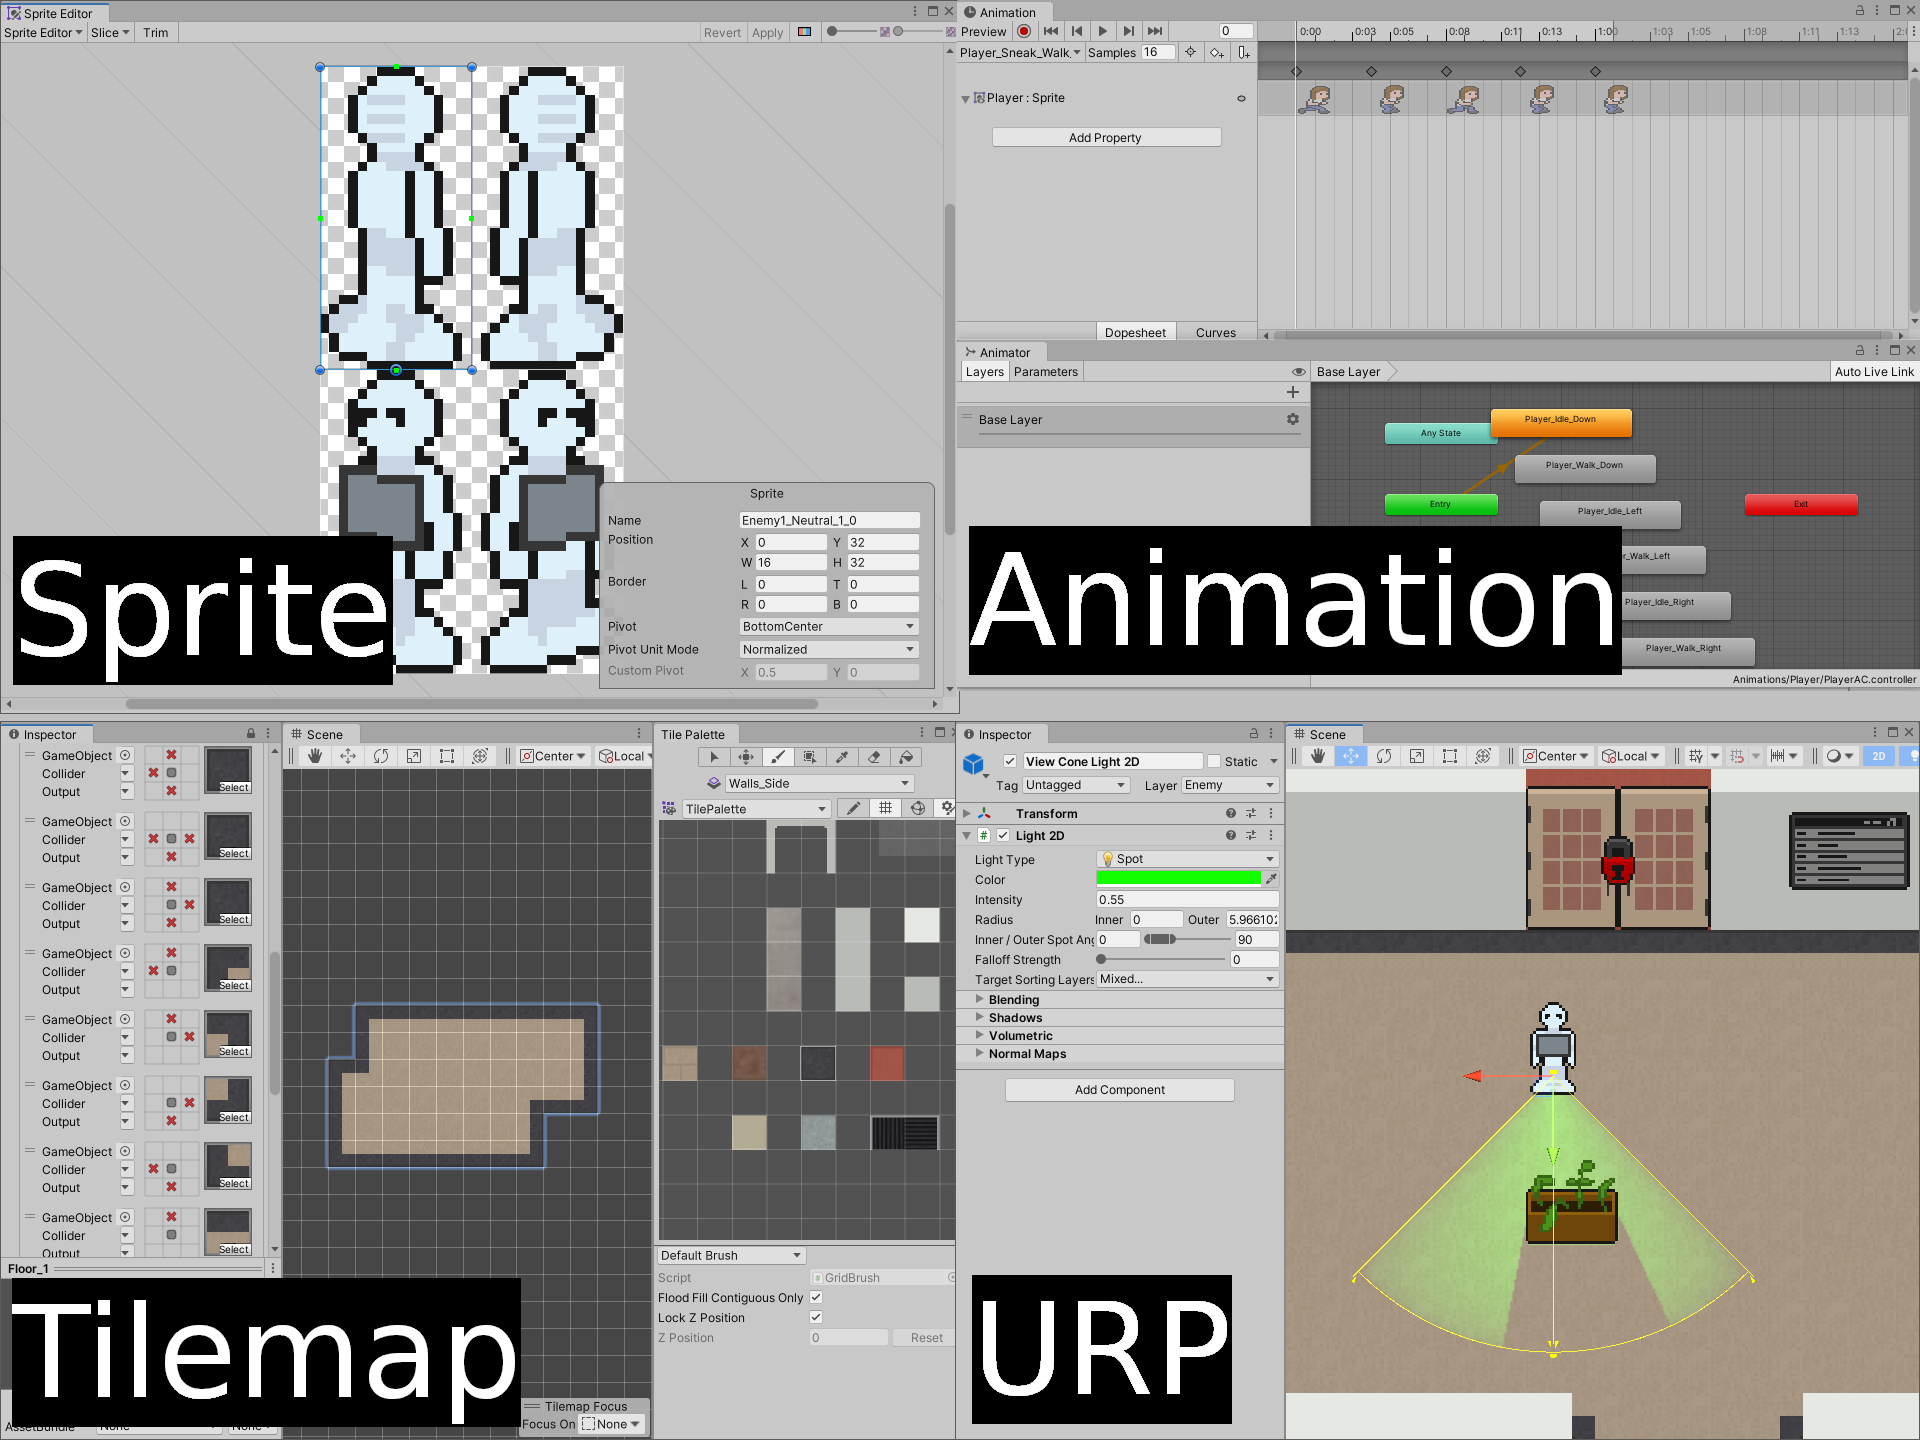
\includegraphics[width=\paperwidth]{Images/UnityShowcase}}
	\end{frame}
	
	% Slide 5 :: Návrh vizuálu
	\section{Návrh – vizuální stránka}
	\begin{frame}{Návrh – vizuální stránka}
		\begin{itemize}\setlength\itemsep{10pt}
			\item Pixel art – jednoduchost, rychlost
			\item Top-down perspektiva
		\end{itemize}
		TODO: Obrázky
	\end{frame}
	
	% Slide 6 :: Návrh žánru
	\section{Návrh – žánr}
	\begin{frame}{Návrh – žánr}
		\begin{itemize}\setlength\itemsep{10pt}
			\item Akční
			\item Stealth
		\end{itemize}
		TODO: Obrázky
	\end{frame}
	
	% Slide 7 :: Návrh FSM
	\section{Návrh – FSM}
	\begin{frame}{Návrh – FSM}
		\begin{figure}[h]
			\centering
			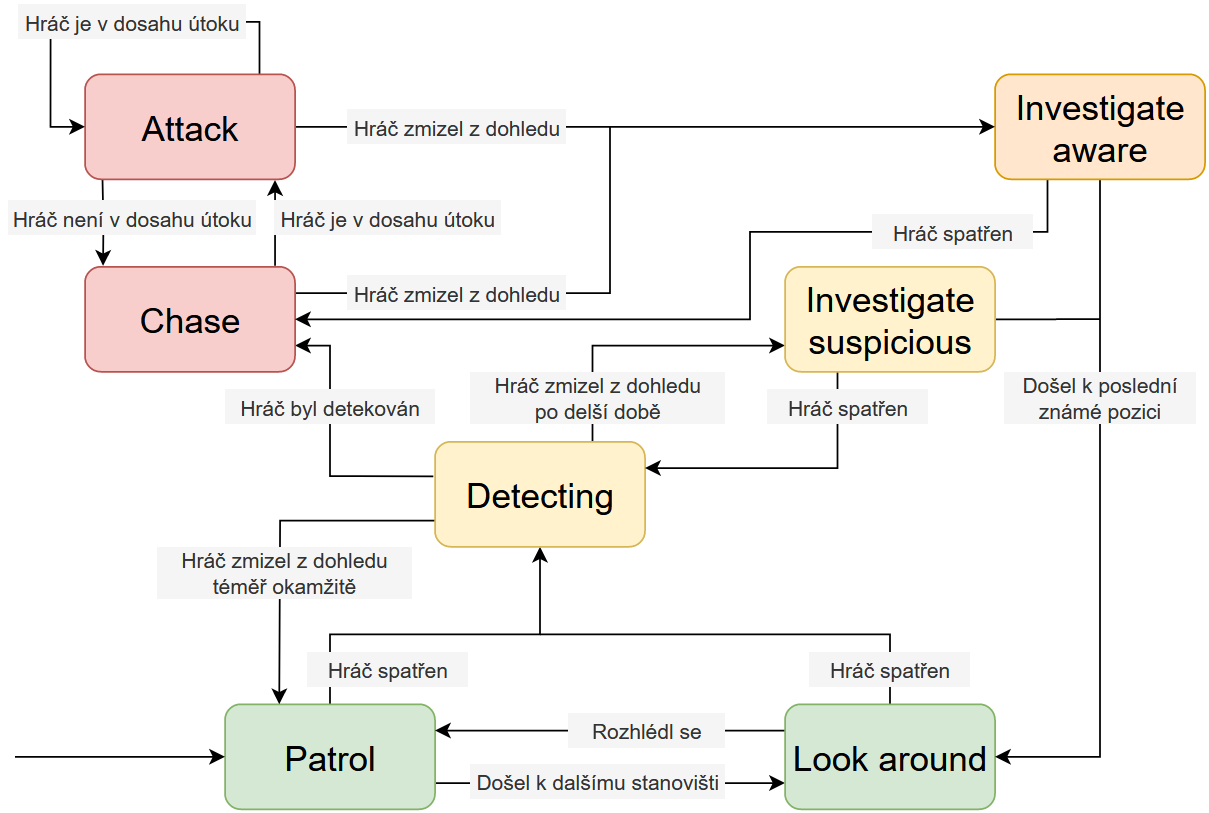
\includegraphics[width=\textwidth]{Images/FSM}
		\end{figure}
	\end{frame}
	
	% Slide 8 :: Implementace
	\section{Implementace}
	\begin{frame}{Implementace}
		\begin{itemize}\setlength\itemsep{10pt}
			\item Grafika – GIMP, problémové animace
			\item Postava hráče – RigidBody2D, FSM
			\item Tvorba mapy – Tilemap, problémy s perspektivou a URP
			\item Jednotka nepřítele – FSM, A*
		\end{itemize}
		TODO: Obrázky
	\end{frame}
	
	% Slide 9 :: Implementace FSM
	\section{Implementace – FSM}
	\begin{frame}{Implementace – FSM}
		TODO: C\# code snippets a/nebo obrázek
	\end{frame}

	% Slide 10 :: Závěr
	\section{Závěr}
	\begin{frame}{Závěr}
		\begin{itemize}\setlength\itemsep{10pt}
			\item $+$ Grafický styl
			\item $+$ Stealth
			\item $+$ FSM
			\item $-$ Audio
			\item $-$ Soubojový systém
			\item $-$ Přístupnost
		\end{itemize}
	\end{frame}

	% Děkuji za pozornost
	{
	\setbeamertemplate{footline}{} % Závěr bez patičky
	\begin{frame}[noframenumbering] % Nepočítat do celkového počtu framů
		Děkuji za pozornost
	\end{frame}
	}
	
\end{document}